\documentclass[12pt,letterpaper]{article}

%-----------------------------
%      PACKAGES & SETUP
%-----------------------------
\usepackage[margin=1in]{geometry}
\usepackage{amsmath,amssymb,amsfonts,bm}
\usepackage{graphicx}
\usepackage{booktabs}
\usepackage{enumitem}
\usepackage{float}
\usepackage{hyperref}
\usepackage{fancyhdr}
\usepackage{cite}
\usepackage{siunitx} % For formatting numbers and units
\usepackage{subcaption}
\usepackage{times}
\usepackage{xspace}
\usepackage{listings}
\usepackage{xcolor}
\usepackage{tabularx} % For better tables

\usepackage[dvipsnames,svgnames,x11names]{xcolor} % full colour set + blends
\definecolor{linkblue}{HTML}{1A4B9B}   
\definecolor{citepink}{HTML}{AA0066}
\definecolor{urlteal}{HTML}{006D6D}

\hypersetup{
  colorlinks = true,
  linkcolor  = linkblue,     
  citecolor  = citepink,     
  urlcolor   = urlteal       
}

\usepackage{verbatim}

\setlength{\headheight}{14.5pt}
\pagestyle{fancy}
\fancyhf{}
\rhead{\thepage}
\lhead{CSE\,291 (SP\,2025) Final Project} % Updated project title

\setlength{\parskip}{6pt}
\setlength{\parindent}{18pt}

% New commands and macros
\newcommand{\R}{\mathbb{R}}
\newcommand{\vel}{\bm{u}}
\newcommand{\pos}{\bm{x}}
\newcommand{\tracerpos}{\bm{p}}
\newcommand{\vortstrength}{\Gamma}
\newcommand{\domainradius}{R_D}
\newcommand{\corevsq}{a_v^2}
\newcommand{\coretsq}{a_t^2}
\newcommand{\xp}{\texttt{xp}\xspace}


\fancypagestyle{ack_footer}{
    \fancyhf{}
    \renewcommand{\headrulewidth}{0pt}
    \renewcommand{\footrulewidth}{0pt}
    \cfoot{
      \scriptsize
      \begin{minipage}[t]{0.95\textwidth}
      \textbf{Acknowledgments:} OpenAI's ChatGPT (model gpt-4o) was utilized to add comments and docstrings to Python functions, explain code implemented by me and ensure its correctness and alignment with equations of motion, and help debug code errors. The outputs from this AI model were modified with major changes. I actively reviewed, tested, and adjusted the generated code and explanations to reflect my own understanding.
      \end{minipage}
    }
}

%% Additional colors and listings setup
\definecolor{lightgray}{gray}{0.95}
\definecolor{darkblue}{rgb}{0.0,0.0,0.5}

\lstset{
    backgroundcolor=\color{lightgray},
    basicstyle=\small\ttfamily,
    keywordstyle=\color{blue}\bfseries,
    commentstyle=\itshape\color{green!40!black},
    stringstyle=\color{red},
    columns=fullflexible,
    breaklines=true,
    frame=single,
    numbers=left,
    numbersep=5pt,
    showstringspaces=false,
    tabsize=4,
    captionpos=b,
    morekeywords={vector,rate,canvas,sphere,cylinder,distant_light,local_light,box,make_trail,trail_radius,trail_color,opacity, SimConfig, njit, prange, ElementwiseKernel, cp, np} % Added some keywords from the new code
}

\begin{document}

%===========================================================
%                     TITLE
%===========================================================
\begin{center}
    {\Large \textbf{Simulation of 2D Point Vortex Dynamics with Passive Tracers \\ in a Circular Domain}}\\[10pt] % Updated Title
    \textbf{Param Somane}\\
    \emph{CSE 291 (Spring 2025) Final Project} % Updated
\end{center}

\vspace{1em}

\begin{abstract}
\noindent
This report details the design and implementation of a numerical simulation for two-dimensional point vortex dynamics within a bounded circular domain. The system models the motion of $N_v$ point vortices, regularized using the Lamb-Oseen model to avoid singularities and provide a finite core structure. Interactions between vortices and their influence on $N_t$ passive tracer particles are simulated. The no-penetration boundary condition at the circular domain wall is enforced using the classical method of images. The equations of motion, comprising a system of ordinary differential equations for vortex and tracer positions, are integrated numerically using an explicit fourth-order Runge-Kutta (RK4) scheme. The implementation supports both CPU-based computation (leveraging NumPy and Numba for JIT compilation) and GPU acceleration (using CuPy), offering flexibility and performance. We describe the governing equations, numerical algorithms, initialization procedures, and visualization techniques. The simulation's fidelity is assessed by monitoring conserved quantities like linear and angular impulse. The project culminates in an animation visualizing the complex, often chaotic, advection of tracers by the vortex flow.
\end{abstract}

%===========================================================
\section{Introduction and Motivation}
%===========================================================
The study of two-dimensional ideal fluid flow provides fundamental insights into a wide range of fluid phenomena. Point vortices, which are idealized singularities of vorticity, serve as elementary building blocks for constructing and understanding complex 2D flows \cite{Saffman1992}. In this model, the vorticity is concentrated at discrete points, and these points move under the influence of the velocity field they collectively generate. While classical point vortices are singular, leading to infinite self-induced velocities, regularized models such as the Lamb-Oseen vortex \cite{Oseen1912} introduces a finite core size, smearing out the vorticity over a small region and yielding more physically realistic interactions, especially at close range.

Confining vortices within a bounded domain introduces interactions with boundaries. For a circular domain, the method of images provides an elegant way to satisfy the no-penetration boundary condition by introducing a system of image vortices outside the domain \cite{MilneThomson1968}. The resulting dynamics can be rich and complex, exhibiting phenomena like vortex pairing, clustering, and chaotic advection.

Passive tracer particles, which are advected by the fluid flow without influencing it, are invaluable tools for visualizing flow patterns. By tracking the trajectories of a large number of tracers, one can gain qualitative and quantitative understanding of mixing, transport, and the overall structure of the velocity field generated by the vortices.

This project implements a simulation of $N_v$ Lamb-Oseen vortices and $N_t$ passive tracers within a circular domain of radius $\domainradius$. The primary goals are:
\begin{itemize}[nosep]
    \item To accurately model the interactions between vortices, including their images.
    \item To simulate the advection of passive tracers by the vortex-induced flow.
    \item To implement an efficient numerical solver using the RK4 method, capable of running on both CPU (with Numba acceleration) and GPU (with CuPy).
    \item To visualize the resulting dynamics and monitor conserved quantities to assess simulation accuracy.
\end{itemize}
The simulation provides a flexible platform for exploring 2D vortex dynamics and serves as an example of a continuum mechanical system simulation as per the project guidelines.

%===========================================================
\section{System Model and Governing Equations}
%===========================================================
\subsection{Domain and Particles}
The system is defined in a two-dimensional circular domain of radius $\domainradius$. It contains two types of particles:
\begin{itemize}
    \item \textbf{Vortices:} $N_v$ point vortices, indexed $k=1, \dots, N_v$. Each vortex $k$ is characterized by its time-dependent position $\pos_k(t) = (x_k(t), y_k(t))$ and its constant circulation strength $\vortstrength_k$.
    \item \textbf{Tracers:} $N_t$ passive tracer particles, indexed $j=1, \dots, N_t$. Each tracer $j$ has a time-dependent position $\tracerpos_j(t) = (p_{jx}(t), p_{jy}(t))$. Tracers are advected by the flow but do not affect it.
\end{itemize}
The state of the system at any time $t$ is described by the collection of all vortex and tracer positions.

\subsection{Velocity Field of a Lamb-Oseen Vortex}
A single Lamb-Oseen vortex of strength $\vortstrength$ with a squared core radius $a^2$, located at the origin, induces a velocity field $\vel(\bm{r}; \vortstrength, a^2)$ at a point $\bm{r}=(x,y)$ given by:
\begin{equation}
    \vel(x,y; \vortstrength, a^2) = \frac{\vortstrength}{2\pi} \frac{1 - e^{-(x^2+y^2)/a^2}}{x^2+y^2} \begin{pmatrix} -y \\ x \end{pmatrix}.
    \label{eq:lamb_oseen_velocity}
\end{equation}
This model regularizes the singularity of a classical point vortex.
\begin{itemize}
    \item As $r = \|\bm{r}\| \to 0$, the velocity approaches that of a solid body rotation: $\vel \to \frac{\vortstrength}{2\pi a^2} \begin{pmatrix} -y \\ x \end{pmatrix}$.
    \item As $r \to \infty$, the velocity approaches that of a potential vortex: $\vel \to \frac{\vortstrength}{2\pi r^2} \begin{pmatrix} -y \\ x \end{pmatrix}$.
\end{itemize}
The implementation uses a factor $f(r^2, a^2) = \frac{1 - e^{-r^2/a^2}}{r^2}$ (with a limit value $1/a^2$ as $r^2 \to 0$ for numerical stability), such that the velocity magnitude is $\frac{|\vortstrength|}{2\pi r} (1 - e^{-r^2/a^2})$.
The Python code defines two distinct squared core radii:
\begin{itemize}
    \item $\corevsq = \texttt{VORTEX\_CORE\_A\_SQ}$: Used when calculating the velocity induced by a vortex on another vortex.
    \item $\coretsq = \texttt{TRACER\_CORE\_A\_SQ}$: Used when calculating the velocity induced by a vortex on a tracer particle.
\end{itemize}
This means the regularization parameter $a^2$ in Eq.~\eqref{eq:lamb_oseen_velocity} effectively depends on the type of particle whose velocity is being computed.

\subsection{Method of Images for Circular Boundary}
To satisfy the no-penetration boundary condition ($\vel \cdot \bm{n} = 0$) on the circular domain wall $r = \domainradius$, the method of images is employed. For each real vortex $k$ at position $\pos_k$ with strength $\vortstrength_k$, an image vortex is introduced at position $\pos_k'$ with strength $\vortstrength_k'$:
\begin{align}
    \pos_k' &= \frac{\domainradius^2}{\|\pos_k\|^2} \pos_k \label{eq:image_pos} \\
    \vortstrength_k' &= -\vortstrength_k \label{eq:image_strength}
\end{align}
A schematic is shown in Figure~\ref{fig:vortex_image_schematic}.

\begin{figure}[H]
    \centering
    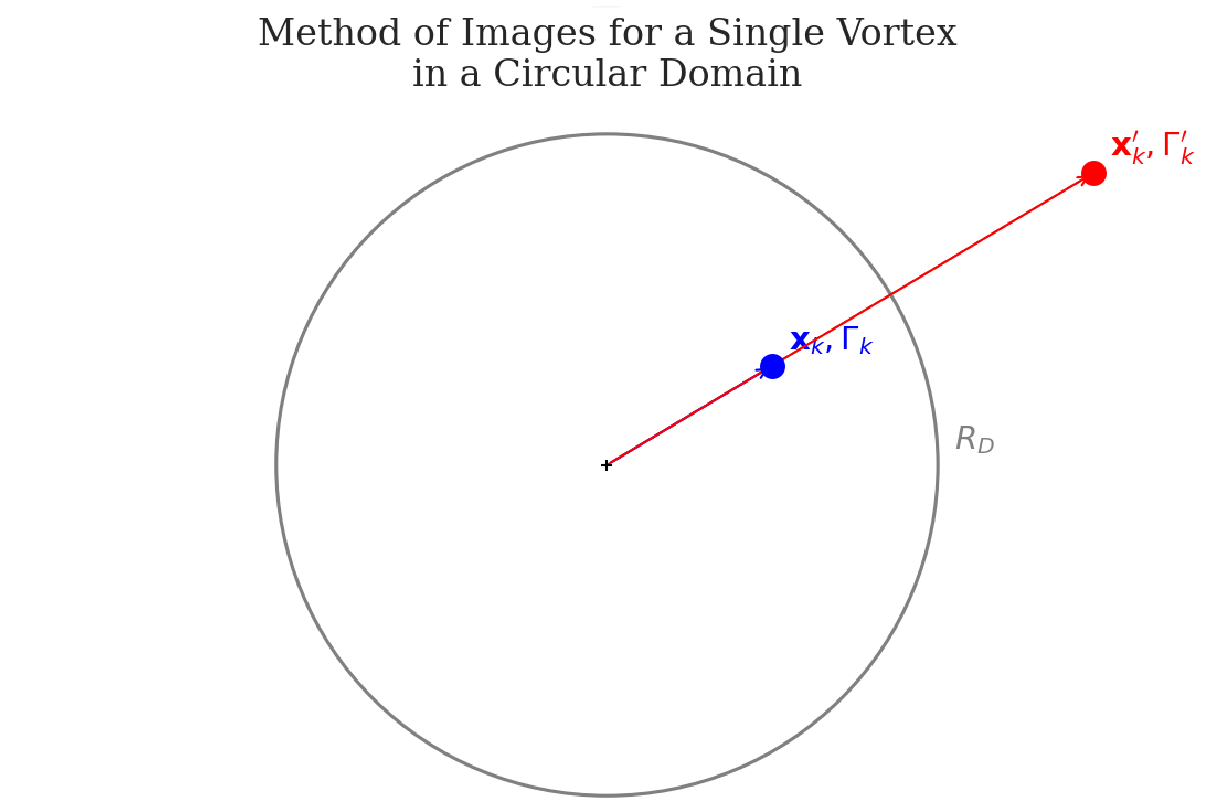
\includegraphics[width=0.8\linewidth]{vortex_image_schematic.png} 
    \caption{Schematic of a vortex $\vortstrength_k$ at position $\pos_k$ within the circular domain of radius $\domainradius$, and its corresponding image vortex $\vortstrength_k'$ at $\pos_k'$ outside the domain. The illustrative real vortex is placed at $(0.5 \domainradius, 0.3 \domainradius)$.}
    \label{fig:vortex_image_schematic}
\end{figure}

Additionally, if the total circulation of real vortices $\vortstrength_{\text{total}} = \sum_{k=1}^{N_v} \vortstrength_k$ is non-zero, a background rotational flow $\vel_{\text{bg}}$ must be added to satisfy the boundary condition:
\begin{equation}
    \vel_{\text{bg}}(\bm{r}; \vortstrength_{\text{total}}, \domainradius) = \frac{\vortstrength_{\text{total}}}{2\pi \domainradius^2} \begin{pmatrix} -y \\ x \end{pmatrix},
    \label{eq:background_flow}
\end{equation}
where $\bm{r}=(x,y)$ is the position where the velocity is evaluated.

\subsection{Equations of Motion}
The velocity of each particle is the sum of velocities induced by all other real vortices, all image vortices, and the background flow.

\textbf{For vortex $i$ at position $\pos_i$}:
\begin{equation}
    \frac{d\pos_i}{dt} = \sum_{\substack{j=1 \\ j \neq i}}^{N_v} \vel(\pos_i - \pos_j; \vortstrength_j, \corevsq) 
                      + \sum_{j=1}^{N_v} \vel(\pos_i - \pos_j'; \vortstrength_j', \corevsq) 
                      + \vel_{\text{bg}}(\pos_i; \vortstrength_{\text{total}}, \domainradius).
    \label{eq:eom_vortex}
\end{equation}
The term $j \neq i$ in the first sum indicates that a vortex does not induce a velocity on itself via its regularized real component (the Lamb-Oseen form is regular at $r=0$, but the standard formulation sums influences from $j \ne i$). The self-image interaction is included in the second sum.

\textbf{For tracer $l$ at position $\tracerpos_l$}:
\begin{equation}
    \frac{d\tracerpos_l}{dt} = \sum_{j=1}^{N_v} \vel(\tracerpos_l - \pos_j; \vortstrength_j, \coretsq) 
                          + \sum_{j=1}^{N_v} \vel(\tracerpos_l - \pos_j'; \vortstrength_j', \coretsq) 
                          + \vel_{\text{bg}}(\tracerpos_l; \vortstrength_{\text{total}}, \domainradius).
    \label{eq:eom_tracer}
\end{equation}
Note the use of $\corevsq$ in Eq.~\eqref{eq:eom_vortex} and $\coretsq$ in Eq.~\eqref{eq:eom_tracer} for the squared core radius parameter in the Lamb-Oseen velocity function $\vel(\cdot)$.

\subsection{Conserved Quantities}
For an unbounded, inviscid 2D flow of point vortices, certain quantities are conserved. In our bounded domain, these may not be strictly conserved due to interactions with the image system and the boundary enforcement. However, monitoring them provides a measure of simulation quality. The primary quantities are:
\begin{itemize}
    \item \textbf{Linear Impulse}: $P_x = \sum_{k=1}^{N_v} \vortstrength_k y_k$ and $P_y = -\sum_{k=1}^{N_v} \vortstrength_k x_k$.
    \item \textbf{Angular Impulse}: $L_z = \sum_{k=1}^{N_v} \vortstrength_k \|\pos_k\|^2 = \sum_{k=1}^{N_v} \vortstrength_k (x_k^2 + y_k^2)$.
\end{itemize}
The total circulation $\vortstrength_{\text{total}} = \sum \vortstrength_k$ is inherently conserved as individual $\vortstrength_k$ are constant. $L_z$ is expected to change if $\vortstrength_{\text{total}} \ne 0$ due to the background flow term.

%===========================================================
\section{Numerical Implementation}
%===========================================================
The system of first-order ordinary differential equations (ODEs) described by Eqs.~\eqref{eq:eom_vortex} and \eqref{eq:eom_tracer} is solved numerically. Let $\bm{Y}(t)$ be the state vector containing all $2(N_v+N_t)$ coordinates of vortices and tracers. The system is $\dot{\bm{Y}} = \bm{F}(\bm{Y}, t)$.

\subsection{Time Integration}
We employ an explicit fourth-order Runge-Kutta (RK4) method to integrate the ODEs. Given the state $\bm{Y}^{(n)}$ at time $t_n$, the state $\bm{Y}^{(n+1)}$ at $t_{n+1} = t_n + \Delta t$ is computed as:
\begin{align*}
 &\bm{k}_1 = \bm{F}\bigl(\bm{Y}^{(n)}, t_n\bigr),\\
 &\bm{k}_2 = \bm{F}\Bigl(\bm{Y}^{(n)}+\tfrac12\,\Delta t\,\bm{k}_1, t_n+\tfrac12\Delta t\Bigr),\\
 &\bm{k}_3 = \bm{F}\Bigl(\bm{Y}^{(n)}+\tfrac12\,\Delta t\,\bm{k}_2, t_n+\tfrac12\Delta t\Bigr),\\
 &\bm{k}_4 = \bm{F}\Bigl(\bm{Y}^{(n)}+\Delta t\,\bm{k}_3, t_n+\Delta t\Bigr),\\[5pt]
 &\bm{Y}^{(n+1)} = \bm{Y}^{(n)} + \tfrac{\Delta t}{6}\,\Bigl(\bm{k}_1+2\bm{k}_2+2\bm{k}_3+\bm{k}_4\Bigr).
\end{align*}
The time step $\Delta t$ is specified by the \texttt{DT} parameter in the \texttt{SimConfig}.

\subsection{Boundary Enforcement}
After each RK4 step, particle positions are checked against the domain boundary $\domainradius$. If a particle at position $\bm{r}_{\text{old}}$ is found outside the domain (i.e., $\|\bm{r}_{\text{old}}\| > \domainradius$), its position is projected back just inside the boundary:
\begin{equation}
    \bm{r}_{\text{new}} = \bm{r}_{\text{old}} \frac{\domainradius (1-\epsilon_{\text{margin}})}{\|\bm{r}_{\text{old}}\|},
\end{equation}
where $\epsilon_{\text{margin}}$ is a small factor (e.g., $0.001$ or $0.0001$ in the code) to prevent particles from sitting exactly on the boundary. This is a simple but effective way to keep particles within the domain.

\subsection{Computational Backend (CPU/GPU)}
The implementation is designed to run on different computational backends for flexibility and performance, managed by the \texttt{SimConfig} object.
\begin{itemize}
    \item \textbf{Array Module (\xp):} A common interface \xp is used, which points to either \texttt{numpy} (for CPU) or \texttt{cupy} (for GPU).
    \item \textbf{Floating Point Precision:} Calculations primarily use 32-bit floating-point numbers (\texttt{float32}) by default, configurable via \texttt{USE\_FLOAT32\_CPU} for the CPU path.
\end{itemize}

\subsubsection{CPU Path}
When \texttt{GPU\_ENABLED} is false:
\begin{itemize}
    \item \textbf{NumPy:} Standard NumPy array operations are used for vectorization where possible.
    \item \textbf{Numba:} For performance-critical loops, such as the summation of velocities and the Lamb-Oseen factor calculation, Numba's \texttt{@njit} (Just-In-Time compilation) decorator is used. Functions like \\\texttt{\_get\_velocities\_induced\_by\_vortices\_cpu\_numba\_impl}, \\\texttt{get\_vortex\_velocities\_cpu\_numba\_impl}, and \\\texttt{\_lamb\_oseen\_factor\_cpu\_numba\_impl} utilize explicit loops, often with \texttt{prange} for potential parallel execution on multi-core CPUs.
\end{itemize}

\subsubsection{GPU Path}
When \texttt{GPU\_ENABLED} is true (and CuPy is available and functional):
\begin{itemize}
    \item \textbf{CuPy:} CuPy provides a NumPy-compatible API for GPU-accelerated computing on NVIDIA GPUs.
    \item \textbf{Custom Kernels:} The Lamb-Oseen factor calculation benefits from a custom CuPy \\ \texttt{ElementwiseKernel} (\texttt{\_lamb\_oseen\_kernel}), which applies the regularized formula efficiently element-wise on the GPU.
    \begin{lstlisting}[language=Python, caption=CuPy ElementwiseKernel for Lamb-Oseen factor (simplified)., basicstyle=\footnotesize\ttfamily, label={lst:cupy_kernel}]
_lamb_oseen_kernel = ElementwiseKernel(
    'float32 r_sq, float32 core_a_sq', 'float32 out',
    r'''
    const float eps = 1e-7f; // Epsilon for numerical stability
    float r_safe = (r_sq < eps) ? eps : r_sq;
    float val = (1.0f - expf(-r_safe / core_a_sq)) / r_safe;
    // Handle limit r_sq -> 0 where factor -> 1/core_a_sq
    out = (r_sq < eps * 10.0f) ? (1.0f / core_a_sq) : val; 
    ''',
    'lamb_oseen'
)
    \end{lstlisting}
    \item \textbf{Vectorized Operations:} Velocity summations (e.g., in \\ \texttt{\_get\_velocities\_induced\_by\_vortices\_xp} and \texttt{get\_vortex\_velocities\_xp}) are expressed using CuPy's vectorized array operations, which are executed in parallel on the GPU. This involves broadcasting and sum reductions across appropriate axes.
\end{itemize}

\subsection{Initialization Details}
The initial state of vortices and tracers is set up by dedicated functions:
\begin{itemize}
    \item \textbf{Vortices (\texttt{initialize\_vortices}):}
    If $N_v \ge 4$, the first four vortices are placed deterministically (e.g., corners of a square) with alternating strengths. Additional vortices are placed randomly within a certain radius, with strengths chosen randomly from a predefined set. If $N_v < 4$, all vortices are placed randomly.
    \item \textbf{Tracers (\texttt{initialize\_tracers}):}
    The placement and initial scalar values of tracers depend on \texttt{TRACER\_COLORING\_MODE}:
    \begin{itemize}
        \item \texttt{group}: Tracers are arranged in \texttt{NUM\_TRACER\_GROUPS} distinct patches, typically circular, distributed around the domain center. Tracers in each group $i$ are assigned a scalar value (e.g., $(i+0.5)/\texttt{NUM\_TRACER\_GROUPS}$) for coloring. An example initial state for this mode is shown in Figure~\ref{fig:initial_config}.
        \item \texttt{scalar}: Tracers are distributed randomly (e.g., within a radius $0.7\domainradius$), and their scalar value is set based on their initial radial position (e.g., $1 - r/(0.7\domainradius)$), creating a radial gradient.
        \item \texttt{speed}: Tracers are placed similarly to `scalar` mode, but their scalar value (used for coloring) is determined by their instantaneous speed during the simulation.
    \end{itemize}
    A global random seed (\texttt{RANDOM\_SEED}) can be set for reproducible initial conditions.
\end{itemize}

\begin{figure}[H]
    \centering
    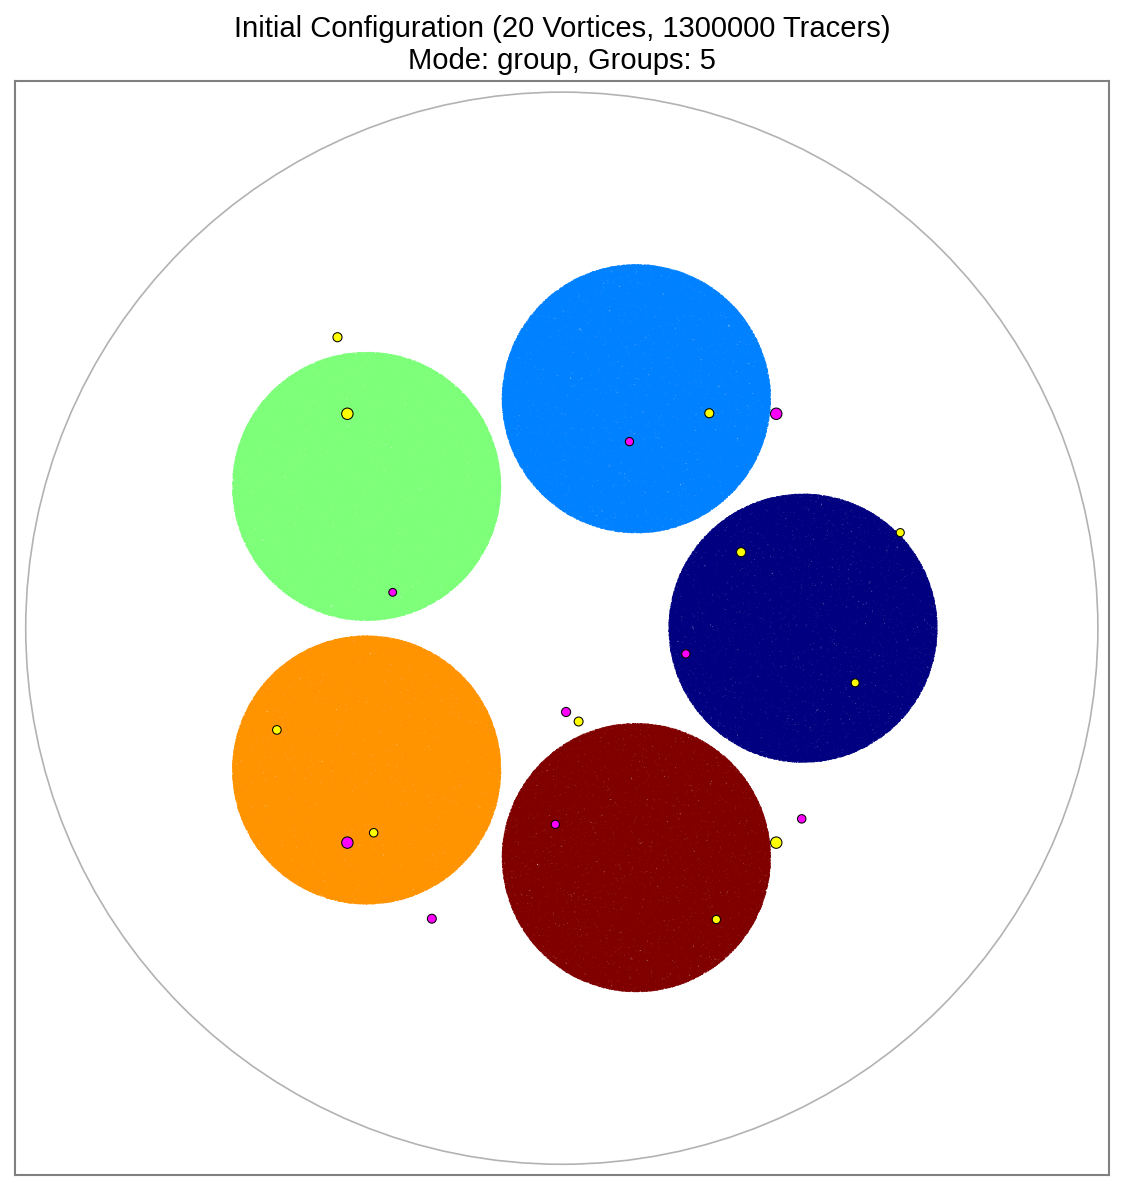
\includegraphics[width=0.61\linewidth]{initial_config_grouped_tracers.png}
    \caption{Example initial configuration of vortices and tracers, generated with $N_v=20$ vortices, $N_t=1,300,000$ tracers, domain radius $\domainradius=1.0$, random seed $42$, and \texttt{TRACER\_COLORING\_MODE='group'} with $5$ tracer groups. Each group is initialized in a distinct patch and assigned a different scalar value for colormap visualization.}
    \label{fig:initial_config}
\end{figure}

%===========================================================
\section{Simulation and Visualization}
%===========================================================
The diffusion, drift, and eventual decay of a viscous counter-rotating vortex pair have been analysed in detail by van Dommelen and Shankar \cite{VanDommelen1995}, providing asymptotic limits that complement the present numerical results.
The simulation evolves the system over a specified \texttt{SIMULATION\_TIME} with time step \texttt{DT}. Data is typically saved at intervals defined by \texttt{PLOT\_INTERVAL} for subsequent animation.

\subsection{Simulation Parameters}
The behavior of the simulation is controlled by parameters in the \texttt{SimConfig} dataclass. Key physical and numerical parameters include:
\begin{itemize}[nosep]
    \item \texttt{N\_VORTICES}, \texttt{N\_TRACERS}: Number of vortices and tracers.
    \item \texttt{DOMAIN\_RADIUS ($\domainradius$)}: Radius of the circular computational domain.
    \item \texttt{SIMULATION\_TIME}, \texttt{DT}: Total simulation duration and integration time step.
    \item \texttt{VORTEX\_CORE\_A\_SQ ($\corevsq$)}, \texttt{TRACER\_CORE\_A\_SQ ($\coretsq$)}: Squared Lamb-Oseen core radii for vortex-vortex and vortex-tracer interactions, respectively.
\end{itemize}
Performance and visualization parameters like \texttt{ANIM\_TRACERS\_MAX} (limits number of tracers in animation for performance) and \texttt{TRACER\_GLOW\_LAYERS} also affect the final output.

\subsection{Visualization}
The simulation results are visualized as an MP4 video generated using Matplotlib's animation capabilities and FFmpeg.
\begin{itemize}
    \item \textbf{Main View:} Shows vortices and tracers within the circular domain.
        \begin{itemize}
            \item Tracers are rendered as small scatter points. Their color is determined by \\ \texttt{TRACER\_COLORING\_MODE} (using \texttt{TRACER\_CMAP}):
                \begin{itemize}
                    \item \texttt{group}/\texttt{scalar}: Color based on pre-assigned scalar values.
                    \item \texttt{speed}: Color based on instantaneous speed, normalized by a global maximum speed observed during the simulation (\texttt{global\_max\_speed\_for\_anim}).
                \end{itemize}
            \item Optional glow effects (\texttt{TRACER\_GLOW\_LAYERS}) can enhance tracer visibility.
            \item Vortices are displayed as larger markers, with color indicating the sign of their strength $\vortstrength_k$ (e.g., yellow for positive, magenta for negative) and size scaled by $|\vortstrength_k|$.
        \end{itemize}
    \item \textbf{Diagnostic Plots:} The animation typically includes subplots showing the evolution of:
        \begin{itemize}
            \item Angular Impulse $L_z(t)$, often as relative deviation $(L_z(t) - L_{z0})/L_{z0}$ if $L_{z0} \neq 0$.
            \item Linear Impulses $P_x(t)$ and $P_y(t)$.
        \end{itemize}
    \item \textbf{Output File:} Specified by \texttt{OUTPUT\_FILENAME}, encoded using \texttt{FFMPEG\_CODEC}.
\end{itemize}

\subsection{Example Simulation Results}
The dynamics of point vortices can be highly complex, leading to chaotic advection of tracers. Depending on initial conditions and vortex strengths, one might observe:
\begin{itemize}
    \item Formation of stable vortex pairs (dipoles) or trios.
    \item Orbiting of weaker vortices around stronger ones.
    \item Merging-like behavior of same-sign vortices (if cores overlap significantly, though point vortices don't truly merge).
    \item Stretching and folding of tracer patches, indicative of chaotic mixing.
\end{itemize}
Example simulations, such as `pv\_group\_1.3M.mp4` (illustrating grouped tracer advection with the `jet` colormap) and `pv\_scalar\_plume\_1.3M.mp4` (showcasing scalar field evolution with the custom `plume` colormap and glow effects), demonstrate these phenomena. These videos, along with the source code, are available at \url{https://github.com/ChestnutKurisu/CSE291D_Final_Project_SP25}. Figure~\ref{fig:simulation_snapshot} shows a representative snapshot from a simulation similar to `pv\_scalar\_plume\_1.3M.mp4`.

\begin{figure}[H]
    \centering
    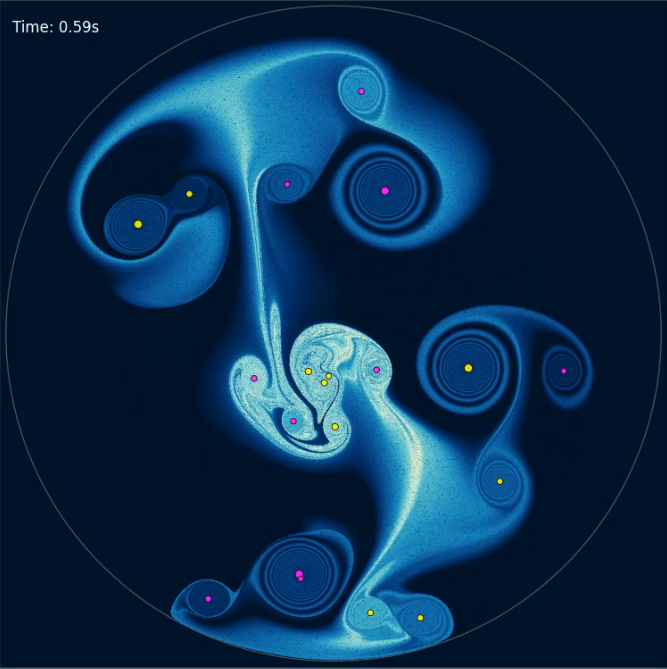
\includegraphics[width=0.65\linewidth]{simulation_snapshot.png} 
    \caption{A snapshot from a simulation run (parameters similar to those for `pv\_scalar\_plume\_1.3M.mp4`: $N_v=20, N_t=1.3 \times 10^6$, `scalar` mode, $t \approx 5.0$\,s), illustrating the advection of tracer particles (shown as small colored dots) by the velocity field generated by the vortices (larger markers). Complex patterns often emerge due to the interactions.}
    \label{fig:simulation_snapshot}
\end{figure}

The conservation of linear and angular impulses serves as a key diagnostic. The plots in Figures~\ref{fig:angular_impulse_plot} and \ref{fig:linear_impulse_plot} show the evolution of these quantities from a representative simulation run detailed in Table~\ref{tab:impulse_params}.
Ideally, for a perfectly symmetric system with $\vortstrength_{\text{total}}=0$ and perfectly reflecting boundaries, $L_z$ and components of $\bm{P}$ would be well-conserved. In practice, numerical errors from RK4 integration, the approximate boundary enforcement (particle projection), and the influence of the background flow (if $\vortstrength_{\text{total}} \neq 0$) can lead to small drifts or oscillations. The observed deviations are generally small, indicating good simulation fidelity.

\begin{table}[H]
    \centering
    \small
    \caption{Parameters for the simulation run that generated the impulse-evolution plots
             (Figures~\ref{fig:angular_impulse_plot} and \ref{fig:linear_impulse_plot}).}
    \label{tab:impulse_params}

    \begin{tabularx}{0.9\textwidth}{X r}
        \toprule
        \textbf{Parameter}                          & \textbf{Value} \\
        \midrule
        Simulation Time                             & 10 s \\
        Time Step (\texttt{DT})                     & 0.002 s \\
        Number of Vortices (\texttt{N\_VORTICES})   & 20 \\
        Squared Vortex Core Radius ($\corevsq$)     & 0.001 \\
        Domain Radius ($\domainradius$)             & 1 \\
        Random Seed                                 & 42 \\
        \midrule
        Initial $L_z$                               & 0.75522 \\
        Final Rel.\ $\Delta L_z / L_{z0}$           & $-4.19 \times 10^{-4}$ \\
        Initial $P_x$                               & 0.76063 \\
        Initial $P_y$                               & $-0.11508$ \\
        Final $P_x$                                 & $-1.266$ \\
        Final $P_y$                                 & 0.28035 \\
        \bottomrule
    \end{tabularx}

    \footnotesize\raggedright
    \vspace{0.5em}
    Note: Impulse conservation depends on the specific vortex configuration (e.g., total strength) and numerical factors. $P_x, P_y$ can change more significantly if there's net drift or rearrangement relative to the origin, especially with image interactions. $L_z$ is generally better conserved if $\Gamma_{\text{total}} \approx 0$.
\end{table}

\begin{figure}[H]
    \centering
    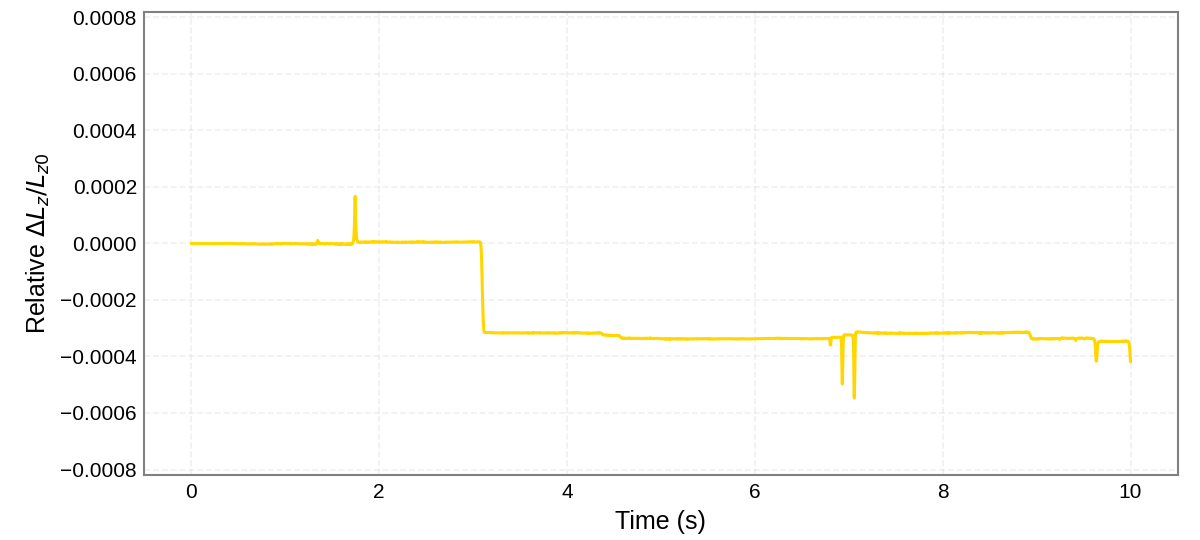
\includegraphics[width=0.86\linewidth]{angular_impulse_plot.png} 
    \caption{Evolution of the relative change in angular impulse $(\Delta L_z / L_{z0})$ over time for the simulation detailed in Table~\ref{tab:impulse_params}. Small fluctuations are typically due to numerical integration and boundary interactions.}
    \label{fig:angular_impulse_plot}
\end{figure}

\begin{figure}[H]
    \centering
    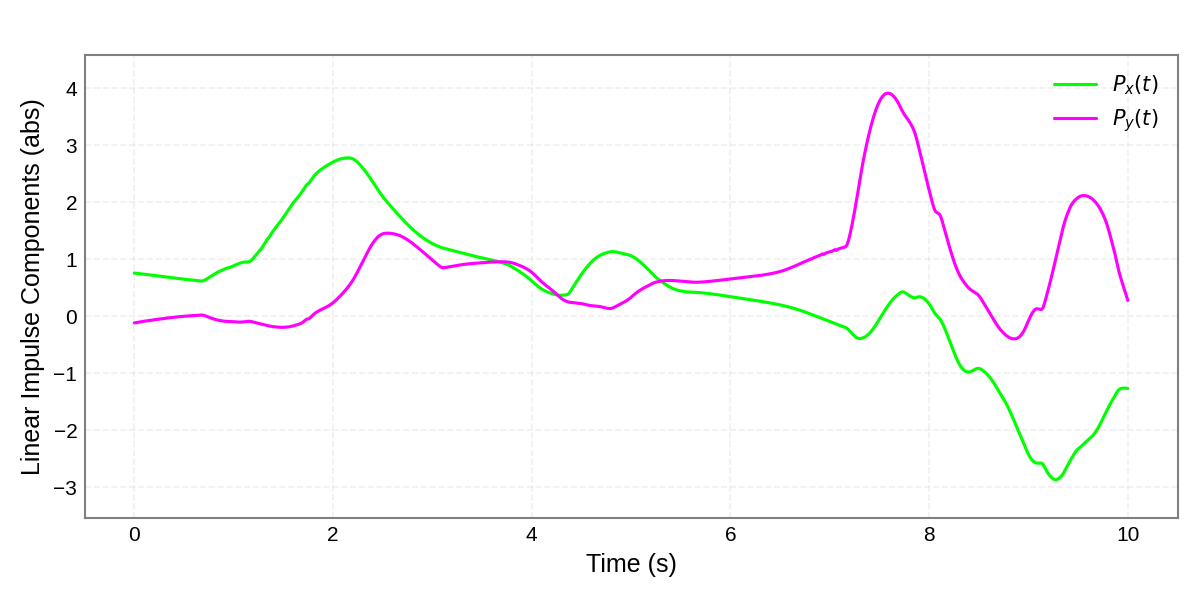
\includegraphics[width=0.86\linewidth]{linear_impulse_plot.png} 
    \caption{Evolution of linear impulses $P_x(t)$ (green) and $P_y(t)$ (magenta) over time for the simulation detailed in Table~\ref{tab:impulse_params}. These quantities are also expected to be nearly conserved, though changes can occur due to interactions with the image system representing the boundary.}
    \label{fig:linear_impulse_plot}
\end{figure}

%===========================================================
\section{Conclusion and Future Work}
%===========================================================
We have successfully developed and implemented a 2D point vortex dynamics simulation. The model incorporates Lamb-Oseen regularization for vortex cores, the method of images for handling a circular boundary, and passive tracer advection for flow visualization. The system's time evolution is computed using an explicit fourth-order Runge-Kutta scheme. A key feature of the implementation is its support for both CPU (accelerated by Numba) and GPU (via CuPy) computation, allowing for efficient simulation of systems with a large number of particles. The generated animations and diagnostic plots of conserved quantities demonstrate the capability of the simulator to capture the complex behavior of vortex flows.

\paragraph{Future Directions.}
Potential extensions and improvements to this work include:
\begin{itemize}[leftmargin=1.8em]
 \item \textbf{More Complex Geometries:} Implementing the method of images or boundary element methods for more complex domain shapes (e.g., airfoils).
 \item \textbf{Viscous Effects:} Incorporating viscous diffusion, for example, by using random walk methods for vortex particle methods or by solving the vorticity-streamfunction formulation of the Navier-Stokes equations.
 \item \textbf{Performance Enhancements:} For very large $N_v$, exploring fast multipole methods or tree codes to accelerate the $O(N_v^2)$ velocity computations.
 \item \textbf{3D Vortex Dynamics:} Extending the simulation to 3D vortex filaments, which involves more complex Biot-Savart law calculations and filament reconnection models.
 \item \textbf{Adaptive Time Stepping:} Implementing adaptive time-stepping in the RK4 solver to improve efficiency and accuracy, especially when vortices undergo close encounters.
 \item \textbf{Interactive Interface:} Developing a graphical user interface for interactive setup of initial conditions and real-time visualization.
\end{itemize}
This project provides a solid foundation for further explorations in computational fluid dynamics and vortex methods.


\appendix
%===========================================================
\section{Details of Numba and CuPy Implementations}
%===========================================================
The computational performance for large numbers of vortices and tracers relies heavily on efficient execution of the velocity calculation routines. This appendix briefly outlines the strategies used for Numba (CPU) and CuPy (GPU).

\subsection{Numba JIT-Compiled Kernels (CPU)}
For the CPU execution path, key functions are JIT-compiled using Numba.
\begin{itemize}
    \item \texttt{\_lamb\_oseen\_factor\_cpu\_numba\_impl}: This function calculates the Lamb-Oseen interaction factor $f(r^2, a^2) = (1 - e^{-r^2/a^2})/r^2$. It typically involves an explicit loop (potentially parallelized with \texttt{prange} if operating on arrays) that iterates through squared distances, applies the formula, and handles the $r^2 \to 0$ limit.
    \item \texttt{\_get\_velocities\_induced\_by\_vortices\_cpu\_numba\_impl} (for tracers) and \\ \texttt{get\_vortex\_velocities\_cpu\_numba\_impl} (for vortices): These functions compute the total velocity for each target particle.
    They generally use nested loops: an outer loop over target particles (parallelized with \texttt{prange}) and an inner loop over source vortices (both real and image). Inside the inner loop, relative positions and squared distances are computed, the Lamb-Oseen factor is found (by calling its Numba version or inlining), and velocity contributions are summed up. This explicit looping, when compiled by Numba, often results in highly efficient machine code, rivaling or exceeding manually vectorized NumPy code for complex access patterns.
\end{itemize}

\subsection{CuPy Kernels and Vectorization (GPU)}
For the GPU execution path, CuPy is used.
\begin{itemize}
    \item \texttt{\_lamb\_oseen\_kernel} (CuPy \texttt{ElementwiseKernel}): As shown in Listing~\ref{lst:cupy_kernel}, this custom kernel applies the Lamb-Oseen factor calculation directly to CuPy arrays on the GPU. This is highly efficient as it minimizes data transfer and leverages massive parallelism.
    \item \texttt{\_get\_velocities\_induced\_by\_vortices\_xp} and \texttt{get\_vortex\_velocities\_xp}: These functions are written using CuPy's NumPy-like API. Operations such as calculating all pairwise differences between target and source positions are achieved using broadcasting:
    \begin{verbatim}
    # E.g., diff_real = target_pos_exp - v_pos_exp
    # target_pos_exp has shape (M, 1, 2)
    # v_pos_exp has shape (1, N, 2)
    # diff_real will have shape (M, N, 2)
    \end{verbatim}
    Subsequent calculations of $r^2$, applying the Lamb-Oseen factor (via the \texttt{ElementwiseKernel}), and summing contributions (e.g., \texttt{xp.sum(..., axis=1)}) are all performed as high-level vectorized operations executed on the GPU. This approach avoids explicit looping in Python and relies on CuPy's underlying CUDA libraries for parallel execution.
\end{itemize}
Both approaches aim to maximize parallelism and data locality appropriate for their respective hardware architectures. The choice between them is managed by the \texttt{GPU\_ENABLED} flag in \texttt{SimConfig}.

% \label{sec:numerical_implementation_gpu_kernel_listing} % Label for the listing in main text. Already used by the listing caption.

%===========================================================
%                      REFERENCES
%===========================================================
\begin{thebibliography}{99}

\bibitem{Saffman1992}
P.~G. Saffman,
\textit{Vortex Dynamics}.
Cambridge University Press, 1993. ISBN 9780511624063.  
\url{https://doi.org/10.1017/CBO9780511624063}

\bibitem{Lamb1932}
H.~Lamb,
\textit{An Introduction to Fluid Dynamics}.
Cambridge University Press, 2000.
\url{https://www.cambridge.org/core/books/an-introduction-to-fluid-dynamics/18AA1576B9C579CE25621E80F9266993}

\bibitem{Oseen1912}
C.~W. Oseen,
``Über die Wirbelbewegung in einer reibenden Flüssigkeit,''  
\textit{Arkiv för Matematik, Astronomi och Fysik}, vol.~7, pp.~14–21, 1912.  
Available via the Swedish Royal Academy scan:  
\url{https://books.google.com/books/about/%C3%9Cber_Wirbelbewegung_in_einer_reibenden.html?hl=da&id=wrCJPgAACAAJ}.

\bibitem{VanDommelen1995}
L.~L. van Dommelen and S.~Shankar,
``Two counter‐rotating diffusing vortices,''
\textit{Physics of Fluids}, vol.~7, no.~4, pp.~808–819, 1995.
\url{https://doi.org/10.1063/1.868604}

\bibitem{MilneThomson1968}
L.~M. Milne-Thomson,
\textit{Theoretical Hydrodynamics}, 5th ed.
Macmillan, 1968.  
\url{https://www.scirp.org/reference/referencespapers?referenceid=1894227}

\bibitem{Batchelor2000}
G.~K. Batchelor,
\textit{An Introduction to Fluid Dynamics}.
Cambridge University Press, 2000 (corrected ed.).  
\url{https://doi.org/10.1017/CBO9780511800955}

\bibitem{NumbaLam2015}
S.~K. Lam, A.~Pitrou, and S.~Seibert,
``Numba: A LLVM-based Python JIT Compiler,''  
in \textit{Proc.\ LLVM-HPC ’15}, Austin, TX, 2015.  
\url{https://doi.org/10.1145/2833157.2833162}

\bibitem{NumbaWebsite2025}
Numba Development Team,
\textit{Numba v0.59.0 Documentation}.  
\url{https://numba.pydata.org/} (accessed 3 Jun 2025).

\bibitem{Okuta2017}
R.~Okuta, Y.~Unno, D.~Nishino, S.~Hido, and C.~Loomis,
``CuPy: A NumPy-Compatible Library for NVIDIA GPU Calculations,''  
in \textit{Proc.\ Workshop on Machine Learning Systems (LearningSys) at NIPS 2017}, Long Beach, CA, 2017.  
\url{http://learningsys.org/nips17/assets/papers/paper_16.pdf}

\bibitem{CuPyWebsite2025}
CuPy Development Team,
\textit{CuPy v13.0.0 Documentation}.  
\url{https://cupy.dev/} (accessed 3 Jun 2025).

\end{thebibliography}

\thispagestyle{ack_footer}

\end{document}